\documentclass[11pt,a4paper]{article}
\usepackage[a4paper,margin=2cm]{geometry}
\usepackage[T1]{fontenc}
\usepackage{lmodern}
\usepackage{microtype}
\usepackage{graphicx}
\usepackage{booktabs}
\usepackage{tabularx}
\usepackage{enumitem}
\usepackage{xcolor}
\usepackage[hidelinks]{hyperref}

\setlist{nosep,leftmargin=1.4em}
\setlength{\parskip}{0.45em}
\setlength{\parindent}{0pt}
\newcommand{\code}[1]{\texttt{\small #1}}
\definecolor{ok}{HTML}{059669}
\definecolor{warn}{HTML}{B45309}
\definecolor{gap}{HTML}{475569}

\title{\textbf{DealProof}\\[0.3em]\large From weeks of manual screening to a sourced decision in minutes}
\author{ContextCon 05 \textperiodcentered{} BITS Pilani \textperiodcentered{} Services, Replaced \textperiodcentered{} Investing track\\
\small Repository: \url{https://github.com/rish-kun/contextcon}}
\date{22 November 2026}

\begin{document}
\maketitle

\begin{abstract}
\noindent Before a buyer commits to a second meeting with a seller, someone has to answer a simple question: \emph{is this company what it says it is?} Today that answer costs tens of hours of analyst time per target and still arrives with claims unchecked. DealProof does the whole first-pass screening as a service. It finds targets that fit a thesis, confirms each company's legal identity, checks every claim against dated records, and returns a clear next step decided by fixed rules. It also drafts the one document request to the seller, which a named person approves before it is sent. A case costs a few rupees in data and model calls. Every fact carries its source and date, and when the records cannot settle a claim, DealProof says so and names the document that would.
\end{abstract}

\section{The problem}
India recorded about 2,658 deals worth roughly \$133 billion in 2025, with mid-market and strategic acquisitions recovering strongly. Every one of those deals starts with the same early screening work: confirming the target exists and is who it claims to be, checking its founders and funding, and testing the claims in its pitch deck. This work is done by hand:
\begin{itemize}
  \item \textbf{It is slow.} An analyst spends 20--40 hours on basic facts for one target. Full diligence on a regulated target commonly runs six to twelve weeks.
  \item \textbf{It is expensive.} Diligence fees typically run 0.5--1.5\% of deal value. The first pass alone costs about INR~40,000--80,000 of analyst time per target at around INR~2,000 an hour.
  \item \textbf{It fails quietly.} Deck claims go unchecked, lookalike company names get mixed up, and missing facts are filled in by guesswork. A wrong fact in a memo is worse than an honest gap.
\end{itemize}
Most targets are screened out, so most of this effort is spent on companies the buyer never acquires. That is where automation pays back fastest.

\section{The use case}
\textbf{The client.} A mid-size Indian 3PL. Its CFO office wants to buy or invest in regional logistics, warehousing and supply-chain technology companies, and today it pays an advisory firm to screen each candidate.

\textbf{A day with DealProof.}
\begin{enumerate}
  \item The associate types the thesis: \emph{``privately held Indian warehousing and supply-chain software companies that serve enterprise customers and show recent expansion''}. DealProof turns it into criteria they can edit and returns a ranked shortlist of real companies. Each one shows ``Fit 82 · 70\% of criteria assessable'', so thin evidence never looks as strong as full evidence.
  \item They open a case on one target and upload the seller's deck. DealProof confirms which legal entity it is, using a domain, registry id or another identifier, never a name alone. It then checks each claim against independent records.
  \item The case returns a disposition and the documents that would settle what is still open. The CFO's manager approves the request email, and it goes to the seller exactly once.
  \item When the seller replies with documents, the affected claims are re-checked. A new version of the assessment shows what changed and why, and the old one is kept.
\end{enumerate}

\textbf{What the analyst sees} (illustration from our product description, not a real company):

\begin{table}[h]
\centering\small
\begin{tabularx}{\linewidth}{@{}p{5.2cm}lX@{}}
\toprule
\textbf{Seller's claim} & \textbf{Status} & \textbf{Why} \\
\midrule
``Incorporated in 2014, based in Pune'' & \textcolor{ok}{\textbf{Supported}} & The company registry record states both. \\
``We employ 250 people'' & \textcolor{gap}{\textbf{Cannot verify}} & A profile-based estimate is lower, but warehouse staff rarely have profiles. Request a dated payroll summary. \\
``Our founder ran operations at a national logistics firm'' & \textcolor{ok}{\textbf{Supported}} & A professional record shows the role and the years. \\
``We opened a new facility in October 2026'' & \textcolor{warn}{\textbf{Partly corroborated}} & A dated announcement describes a planned facility; nothing shows it operating. \\
``We have no debt'' & \textcolor{gap}{\textbf{Cannot verify}} & A registered charge shows security was given, not that money is owed. Request lender statements. \\
\bottomrule
\end{tabularx}
\end{table}
\textbf{Outcome:} \emph{Investigate further}: a strong fit with three claims still open, and a request for three documents waiting for the manager's approval. An analyst would reach the same conclusion after a day or more of work. DealProof reaches it in minutes, with every line traceable.

\textbf{On live data.} We ran the full pipeline on the logistics thesis. It shortlisted 25 real companies, then verified a warehouse-management software company against 9 claims taken from its own website. Customer counts, certifications and partnerships are not in public records, so 8 of those claims came back \emph{cannot verify}, each naming the document to request. Financials were marked ``not assessed'' rather than estimated. Nothing was sent to the company.

\section{The solution}
\begin{table}[h]
\centering\small
\begin{tabularx}{\linewidth}{@{}lX@{}}
\toprule
\textbf{Input} & A thesis in plain words; or a company name and website with an optional seller deck; or a business profile, to find investors whose dated deals fit it. \\
\textbf{Output} & A screening case: confirmed identity; a claim ledger where each claim has a status, source link, exact passage or field, and date; five separate judgments; one disposition (prioritise, investigate further, deprioritise, cannot assess) with the rule that decided it; an approved request to the seller; the cost of every call. \\
\textbf{Pass mark} & Correct identity, or \emph{cannot assess} for a lookalike; each claim has the expected status, with \emph{cannot verify} where no source settles it; no duplicate merged or counted twice; no email without approval or sent twice; within budget and correct after a kill and restart. \\
\bottomrule
\end{tabularx}
\end{table}

Four principles make the output something a firm can sign off on:
\begin{enumerate}
  \item \textbf{Rules decide, the model extracts.} Claude only reads text and drafts prose. Every status and disposition comes from pure, versioned rules, so the same evidence always gives the same answer.
  \item \textbf{Every fact has a source and a date.} An extracted value must appear in its source passage, or it is thrown away.
  \item \textbf{Identity first.} Nothing attaches to a company on a name alone. If identity is unclear, the case says \emph{cannot assess} rather than guessing.
  \item \textbf{Gaps are stated, not filled.} Silence in a source is never treated as contradiction, and missing evidence never counts against a company.
\end{enumerate}

\begin{figure}[t]
\centering
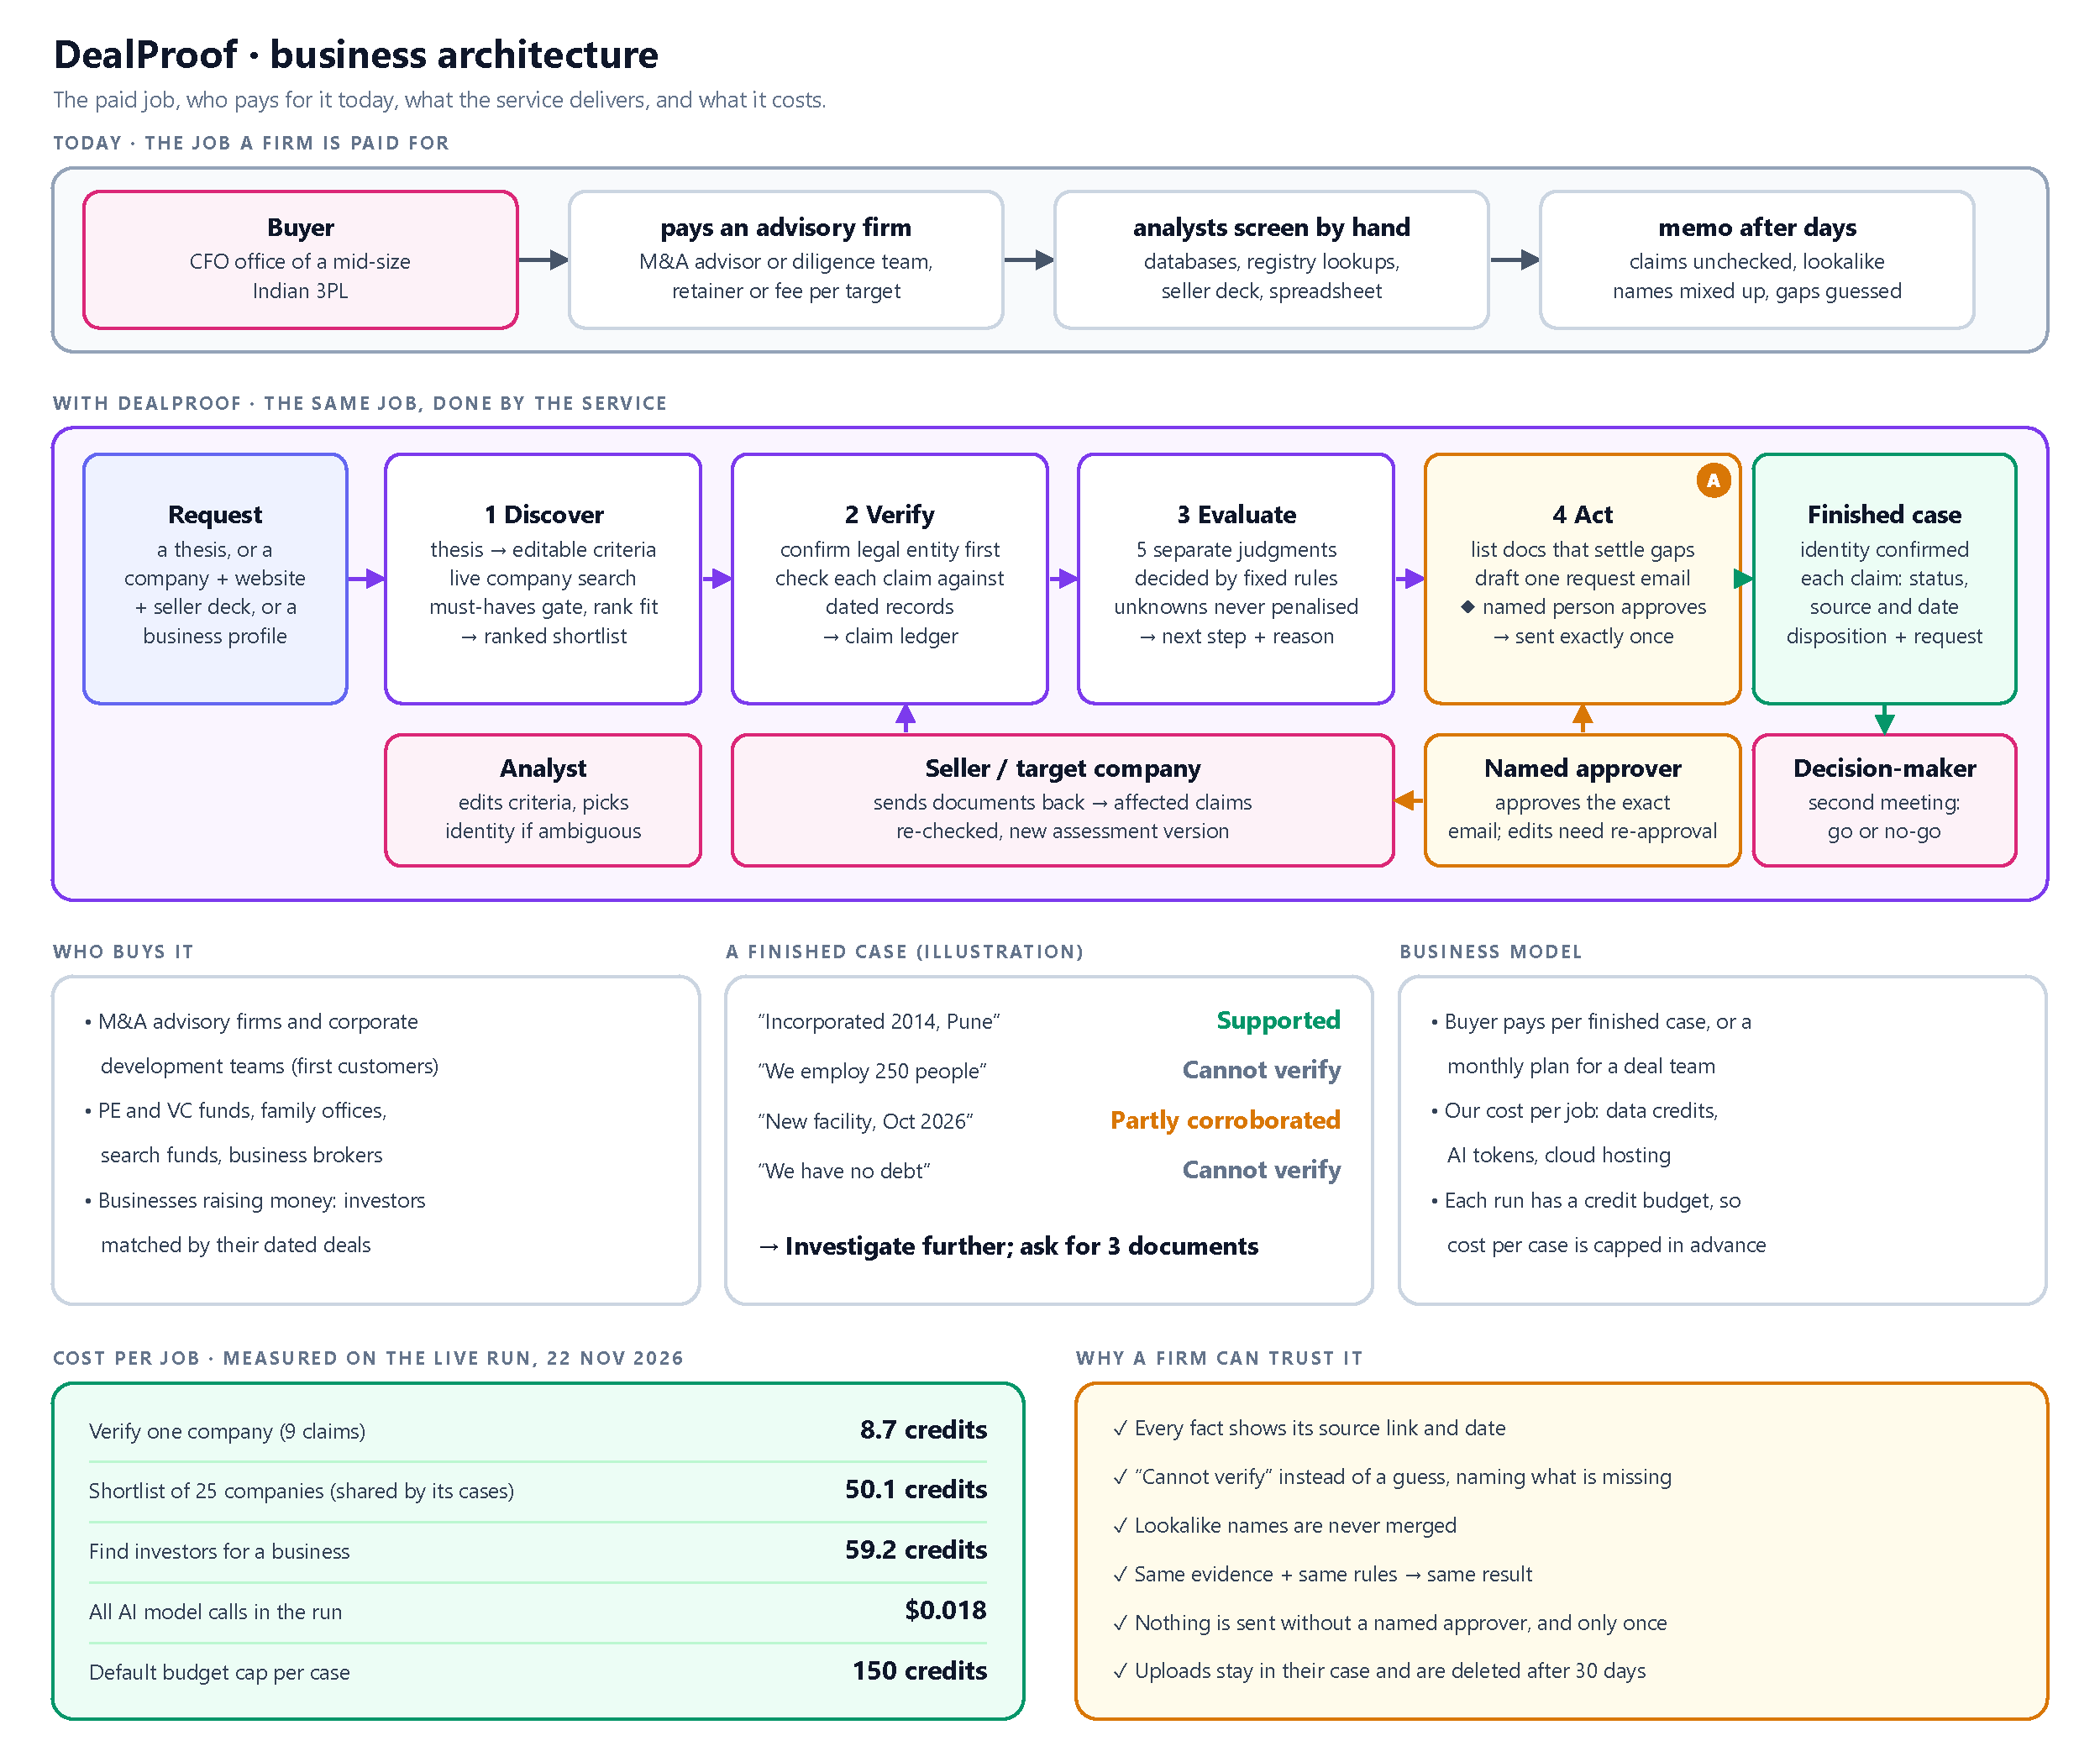
\includegraphics[width=\linewidth]{figures/business-architecture.pdf}
\caption{Business architecture: the job today, the same job done by DealProof, the people in the loop, who buys it, measured cost and trust controls.}
\label{fig:business}
\end{figure}

\section{Architecture}
Figure~\ref{fig:business} shows the service from the buyer's side; Figure~\ref{fig:technical} shows how it is built, in four layers:
\begin{enumerate}
  \item \textbf{Web app} (Next.js, Cloud Run): discovery, case pages, approvals queue, live run progress.
  \item \textbf{API and job engine} (FastAPI, Cloud Run): every request becomes a \emph{Run} of small, idempotent \emph{Steps} stored in Postgres, flowing through Discover, Verify, Evaluate and Act.
  \item \textbf{Call gateway}: every paid call passes through one path: cache, then budget reservation and an attempt log, then the call with retries, then the cost record.
  \item \textbf{Sources and storage}: Crustdata (companies, people, jobs, live web search and fetch), Claude Haiku, Resend for email, Neon Postgres, and a private Cloud Storage bucket.
\end{enumerate}

\begin{figure}[t]
\centering
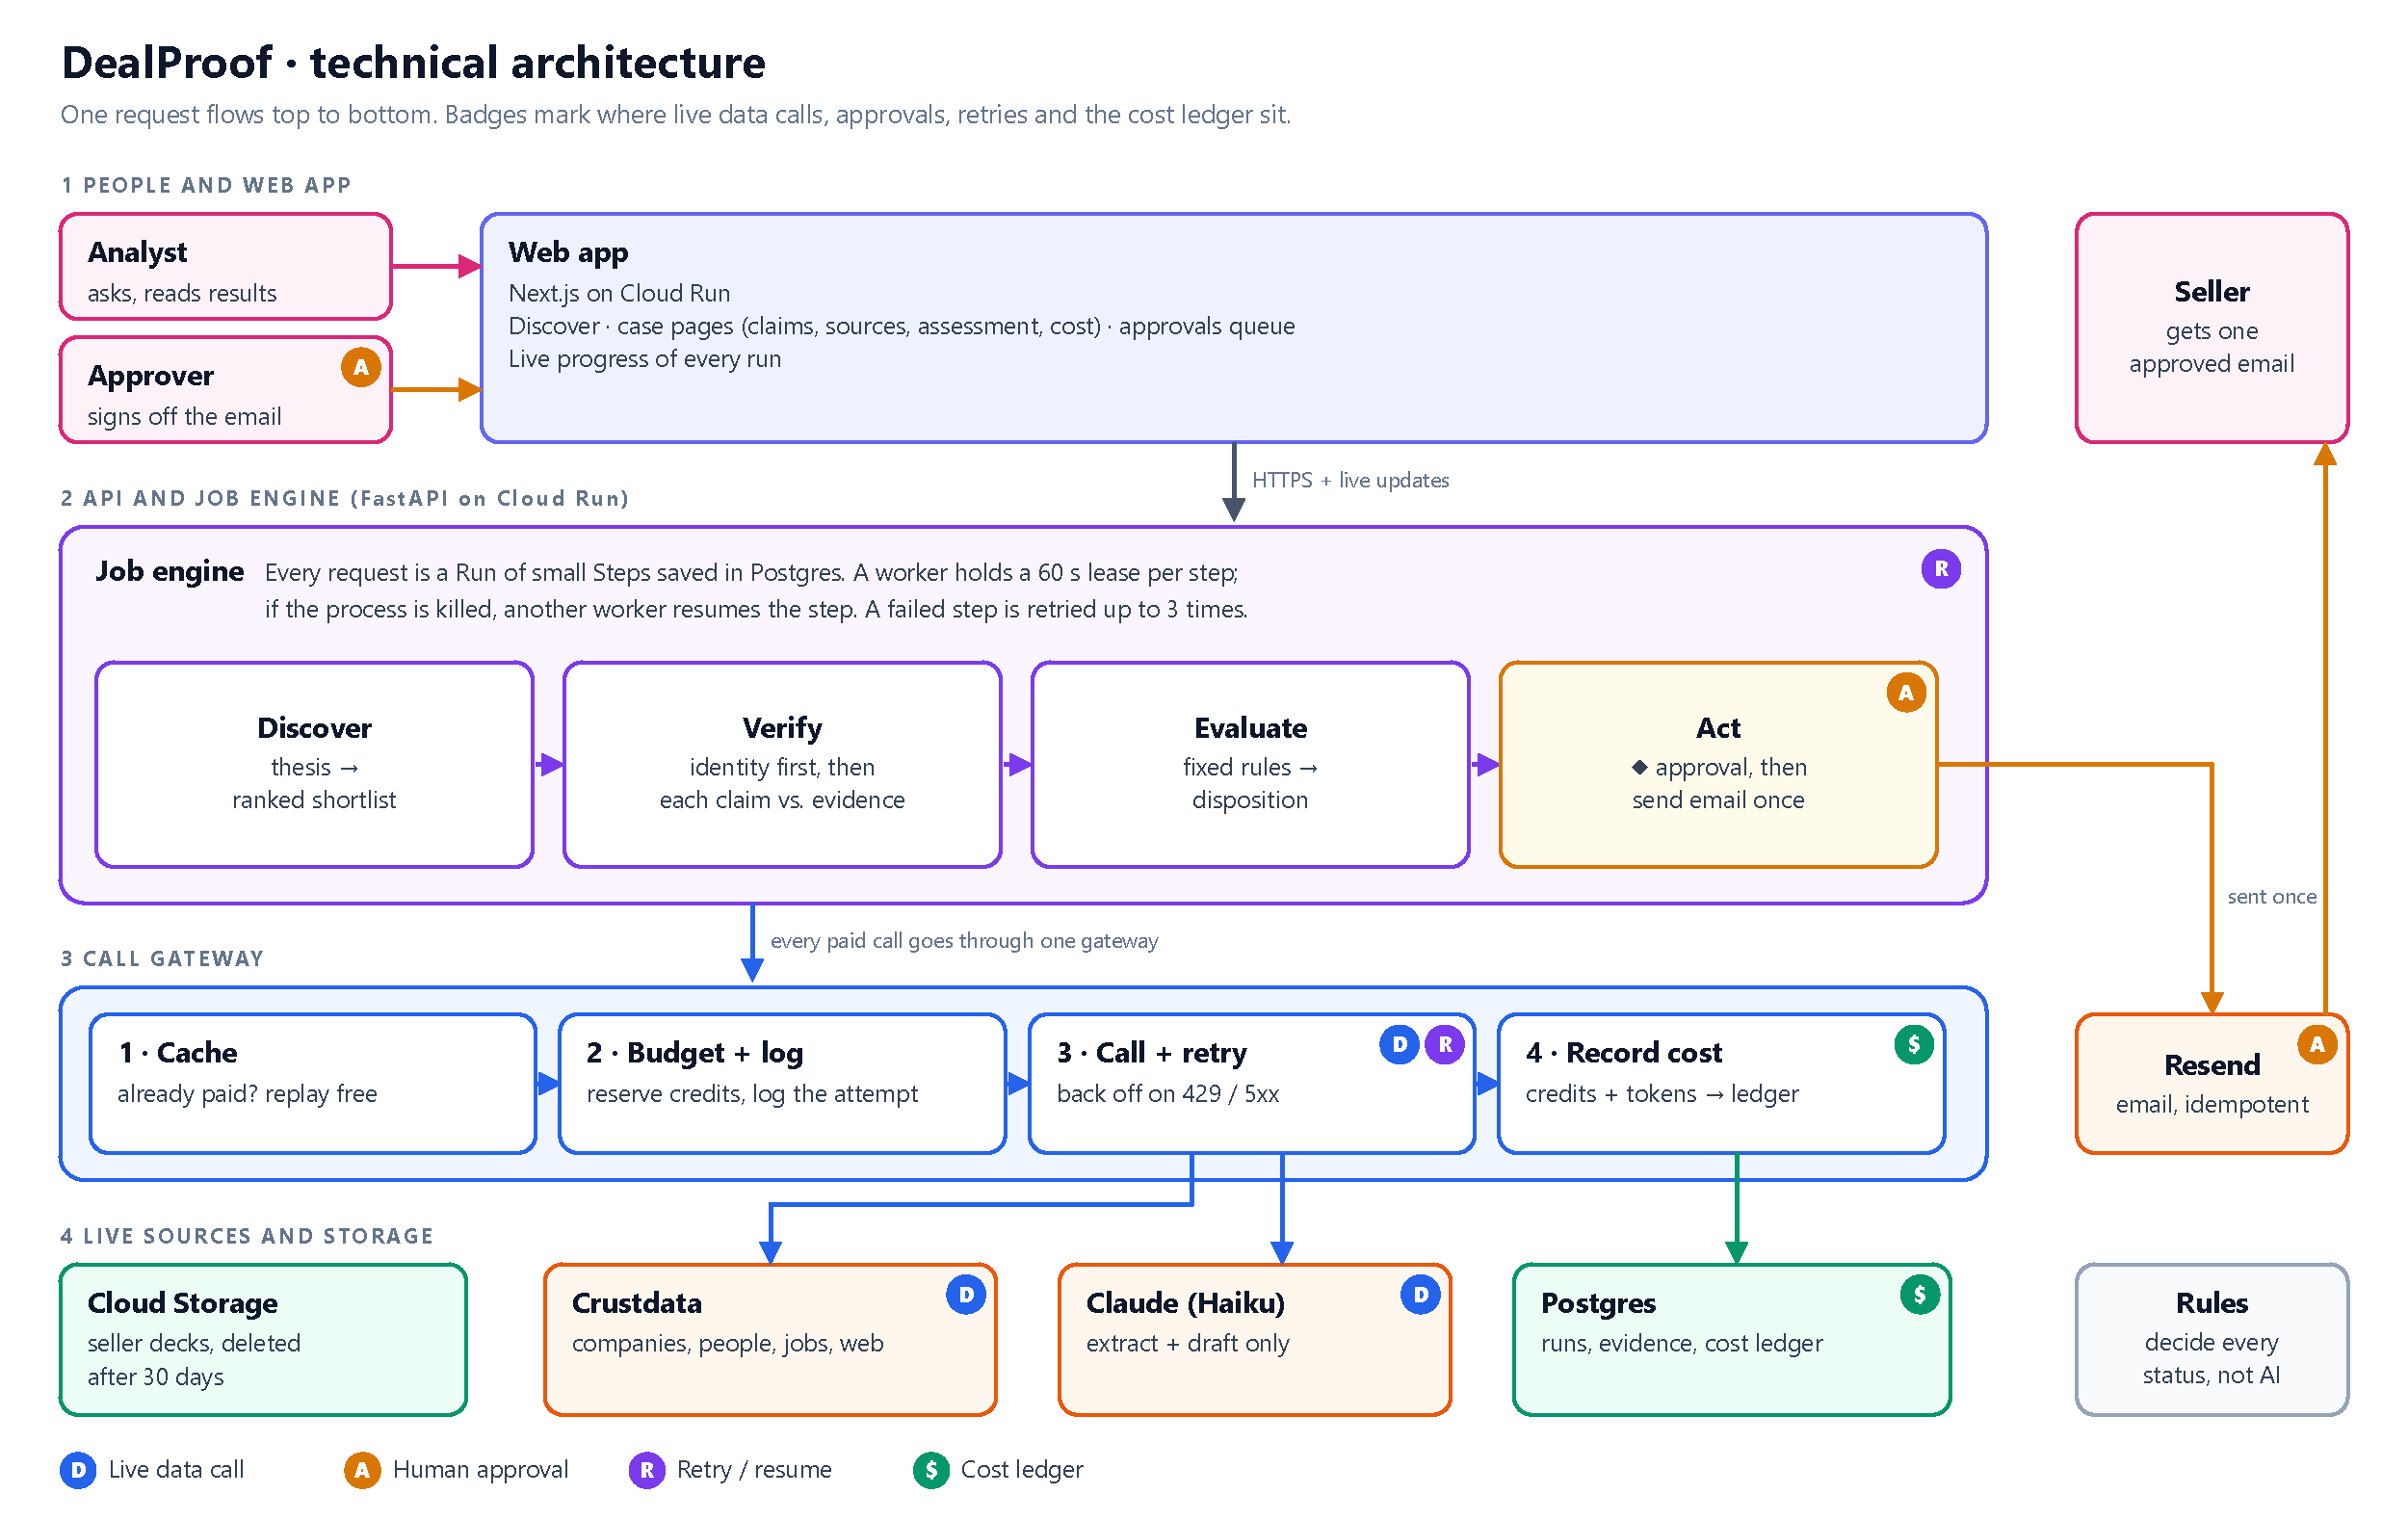
\includegraphics[width=\linewidth]{figures/technical-architecture.pdf}
\caption{Technical architecture. Badges mark live data calls (D), human approval (A), retry and resume points (R), and the cost ledger (\$).}
\label{fig:technical}
\end{figure}

\section{Implementation}
\textbf{Survives a crash.} Workers claim steps with \code{SELECT ... FOR UPDATE SKIP LOCKED} and a 60-second lease that carries a fencing token. If the process is killed, another worker picks the step up. Completed calls replay from cache for free, so nothing is paid for twice.

\textbf{Retries without hidden cost.} HTTP calls retry on rate limits, server errors and timeouts with exponential backoff (Crustdata up to 3 times, Claude up to 2). Each retry is logged as its own attempt. A step that still fails shows as \emph{not checked}, never as a clean result.

\textbf{Every rupee accounted for.} Each call writes an attempt row before it runs and a cost row (credits, tokens, USD) after it. A lost usage figure is stored as \emph{unknown}, not zero. Each case has a credit budget, and checks beyond it become \emph{not checked: budget reached}.

\textbf{Approval that cannot be bypassed.} Approval binds to one immutable email revision, and any edit needs a new approval. A unique send key is stored before sending and passed to the provider as its idempotency key, so a retry or a crash cannot send the email twice.

\textbf{Personal data stays contained.} Uploads are used only for their case, stripped of personal details, and deleted after 30 days with everything derived from them. Search queries use public terms only, never confidential claim text.

\textbf{Tested.} About 770 automated tests cover every claim status and disposition rule, lookalike identities, copied press releases, concurrent sends, lost provider responses and lease reclaim after a crash.

\section{Impact and economics}
\begin{table}[h]
\centering\small
\begin{tabularx}{\linewidth}{@{}Xll@{}}
\toprule
 & \textbf{Today (analyst)} & \textbf{DealProof} \\
\midrule
Time for a first-pass screen & 20--40 hours & minutes, plus review \\
Cost of that screen & INR~40,000--80,000 & data + model: a few rupees \\
Claims checked & whatever time allows & every claim, with source and date \\
Unknowns & often guessed & named, with the document to request \\
\bottomrule
\end{tabularx}
\end{table}

\textbf{Measured cost.} Verifying one company with 9 claims used 8.7 Crustdata credits. A shortlist of 25 companies used 50.1 credits, shared across every case opened from it. All model calls in the run cost \$0.018. At about a cent per credit, data and model costs come to under a rupee per claim checked.

\textbf{Price and margin.} At a proposed INR~20,000 per screened target, or a monthly plan for a deal team, DealProof costs a buyer a quarter to a half of one analyst's first pass. Variable costs stay below 1\% of the price.

\textbf{Who buys first.} Mid-market PE firms (about 300 are active in India) and corporate development teams screen many targets a year and already pay for diligence. Search funds, family offices and roll-up operators follow. Businesses raising money use the reverse flow to find investors whose dated deals match them.

\section{Limitations and future work}
\begin{itemize}
  \item \textbf{Coverage:} Indian courts, IP registries and the charges register have no open API, so litigation and debt claims show as \emph{cannot verify} with the document that would settle them. Dedicated connectors are next.
  \item \textbf{Financials:} private company accounts are rarely public. The financial judgment is ``not assessed'' unless the seller supplies statements.
  \item \textbf{Time limit:} runs are bounded by per-call timeouts and step attempts, but there is no single wall-clock deadline per run yet.
  \item \textbf{Next:} official MCA master data for identity, cross-checks between seller documents, peer benchmarking, comparing several targets under one thesis, and alerts when a monitored company's evidence changes.
\end{itemize}

\section{Conclusion}
DealProof turns the most repetitive part of deal-making into a service that is faster, cheaper and more honest than the manual version. Every fact is sourced and dated, gaps are named instead of guessed, rules decide instead of model opinion, and a person approves the one action that cannot be undone. For a buyer, that means walking into the second meeting knowing which claims hold, which do not, and exactly what to ask for.

\end{document}
